% !TeX root = ../../../thesis.tex

\subsection{Orthogonal Sequences}
\label{subsec:orthogonal-sequences}

Orthogonal sequences, also known as Walsh-Hadamard sequences, are sequences which are created using a Hadamard matrix.
Hadamard matrices are square $n \times n$ matrices which are recursively generated.
Starting with a $1 \times 1$ matrix: 
		$H_{1} = \begin{bmatrix} 1 \end{bmatrix}$, then 
		$H_{2} = \begin{bmatrix} 1 & 1 \\ 1 & -1 \end{bmatrix}$.
See \autoref{eq:hadamard-matrix-creation} for a general recursive formula to generate other ranks of Hadamard matrices \cite{714616}.

\begin{equation}
	H_{2n} = 
	\begin{bmatrix} 
		H_n & H_n \\ 
		H_n & -H_n 
	\end{bmatrix}
	\label{eq:hadamard-matrix-creation}
\end{equation}

The matrix can also be filled with binary values: $0$ and $1$. In that case the general recursive formula is stated in \autoref{eq:hadamard-matrix-creation-bin}. 

\begin{equation}
	H_{2n} = 
	\begin{bmatrix} 
		H_n & H_n \\ 
		H_n & \overline{H_n}
	\end{bmatrix}
	\label{eq:hadamard-matrix-creation-bin}
\end{equation}




The Hadamard matrix has the property that every row in the matrix, apart from the first row, is orthogonal to every other row, meaning that the cross-correlation is zero.
And apart from the first row, all other rows have the exact same number of $+1$s and $-1$s, meaning that the codes are balanced.

Hadamard matrices exist for every power of $2$, so the code length is also a power of $2$.
For $\tau = 0$, the cross-correlation is $0$, but when $\tau \neq 0$ not all the rows have a zero cross-correlation with all other rows.
All rows of the matrix have the property that the autocorrelation at $\tau = 0$ is equal to $L$.
But when $\tau \neq 0$, undesirable behavior occurs as can be seen in \autoref{fig:autocorr-hadamard}.
The autocorrelation function has several high peaks where only one is desired, namely at $\tau = 0$.
This means that if an LED is turned on by a user and it start modulating its code, to transmit that this LED is on, but the smart-meter does not know when in time the start of this code is, because the smart-meter and the LEDs are not synchronized.
So the smart-meter will get false-positives for data.
If there was a way that the smart-meters and all the LEDs could be synchronized with each other, the orthogonal codes will work.

\begin{figure}[t]
	\centering
	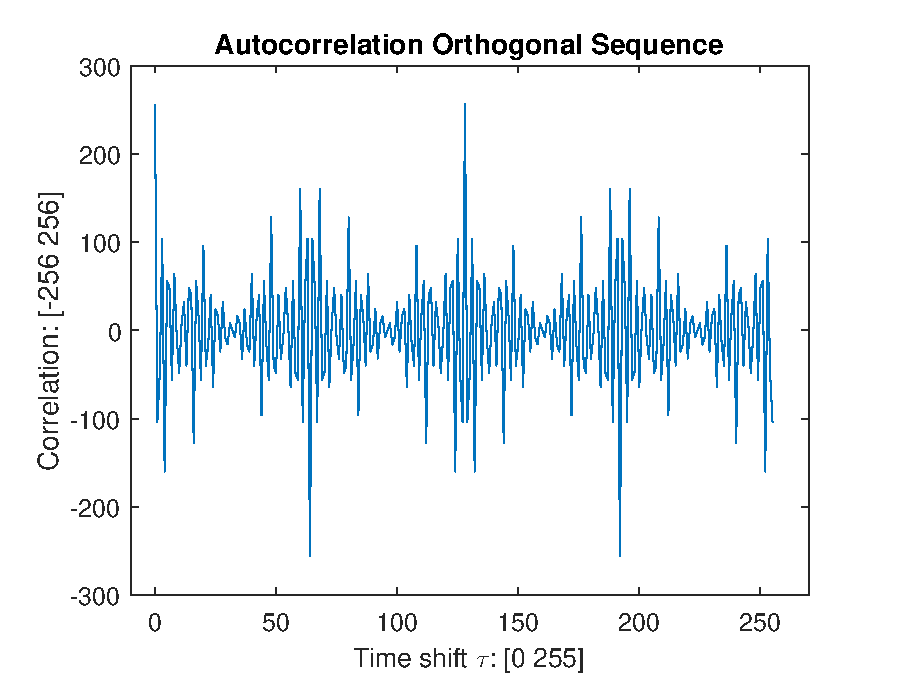
\includegraphics[width=\textwidth]{chapters/cdma-chapters/codes/autocorr-hadamard.eps}
	\caption{Autocorrelation of orthogonal sequence with row index 120 of length 256.}
	\label{fig:autocorr-hadamard}
\end{figure}





To conclude: the entire set of orthogonal codes of length $L$, has $L - 1$ codes in the set which does make it a scalable set.
But the auto- and cross-correlation only have the desired properties when the codes are sent synchronously. 




\subsubsection{Cyclically Orthogonal Walsh Hadamard Codes}

To overcome the problem when sending orthogonal codes in an asynchronous manner, a subset of the orthogonal codes have been identified that are still orthogonal to each other, no matter how these codes are time-shifted with respect to each other.

In \cite{1182447} the authors proved that an Hadamard matrix of size $2^P$ could be divided into $P + 1$ subsets of rows, where one row could be selected giving $P + 1$ orthogonal rows for each time-shift $\tau$.
In other words, this subset of rows have a cross-correlation of zero, for every time-shift $\tau$.
These codes are called Cyclically Orthogonal Walsh Hadamard Codes (COWHC).
With code length $L$ there are $\log_2 L$ codes in the set, which makes these codes not scalable \cite{1182447}. 
Also the auto-correlation does not have a clear peak to identify the code, because these codes are an unmodified subset of the original orthogonal sequences.
For these sequences the auto-correlation has already been shown in \autoref{fig:autocorr-hadamard}.

These codes suffer from the same auto-correlation problems as the normal Orthogonal codes as described in \autoref{subsec:orthogonal-sequences} and they have the additional drawback that they are less scalable.